\documentclass[11pt]{beamer}
\usetheme{Madrid}
\usecolortheme{crane}
\graphicspath{{images/}{./}} % Specifies where to look for included images (trailing slash required)

\title{Building a miniHPC}
\author{Dr Jannetta S Steyn, Dr Colin Sauze, Dr Abhishek Dasgupta}
\institute[NCL, UC, NOC]{Newcastle University, University of Cambridge, National Oceanic Centre\\ \smallskip \textit{jannetta.steyn@newcastle.ac.uk}}
\date[\today]{General set of Slides \\ \today}
\begin{document}
\begin{frame}[plain]
    \maketitle
    	\begin{figure}
    	
\includegraphics[height=10mm]{NOC.png}
    	
\includegraphics[height=10mm]{NCL.png}
		
\includegraphics[height=10mm]{OFFLINE.png}
		
\includegraphics[height=10mm]{SSI.png}
    \end{figure}
\end{frame}
\begin{frame}{Meet Pixie}
	\begin{figure}
		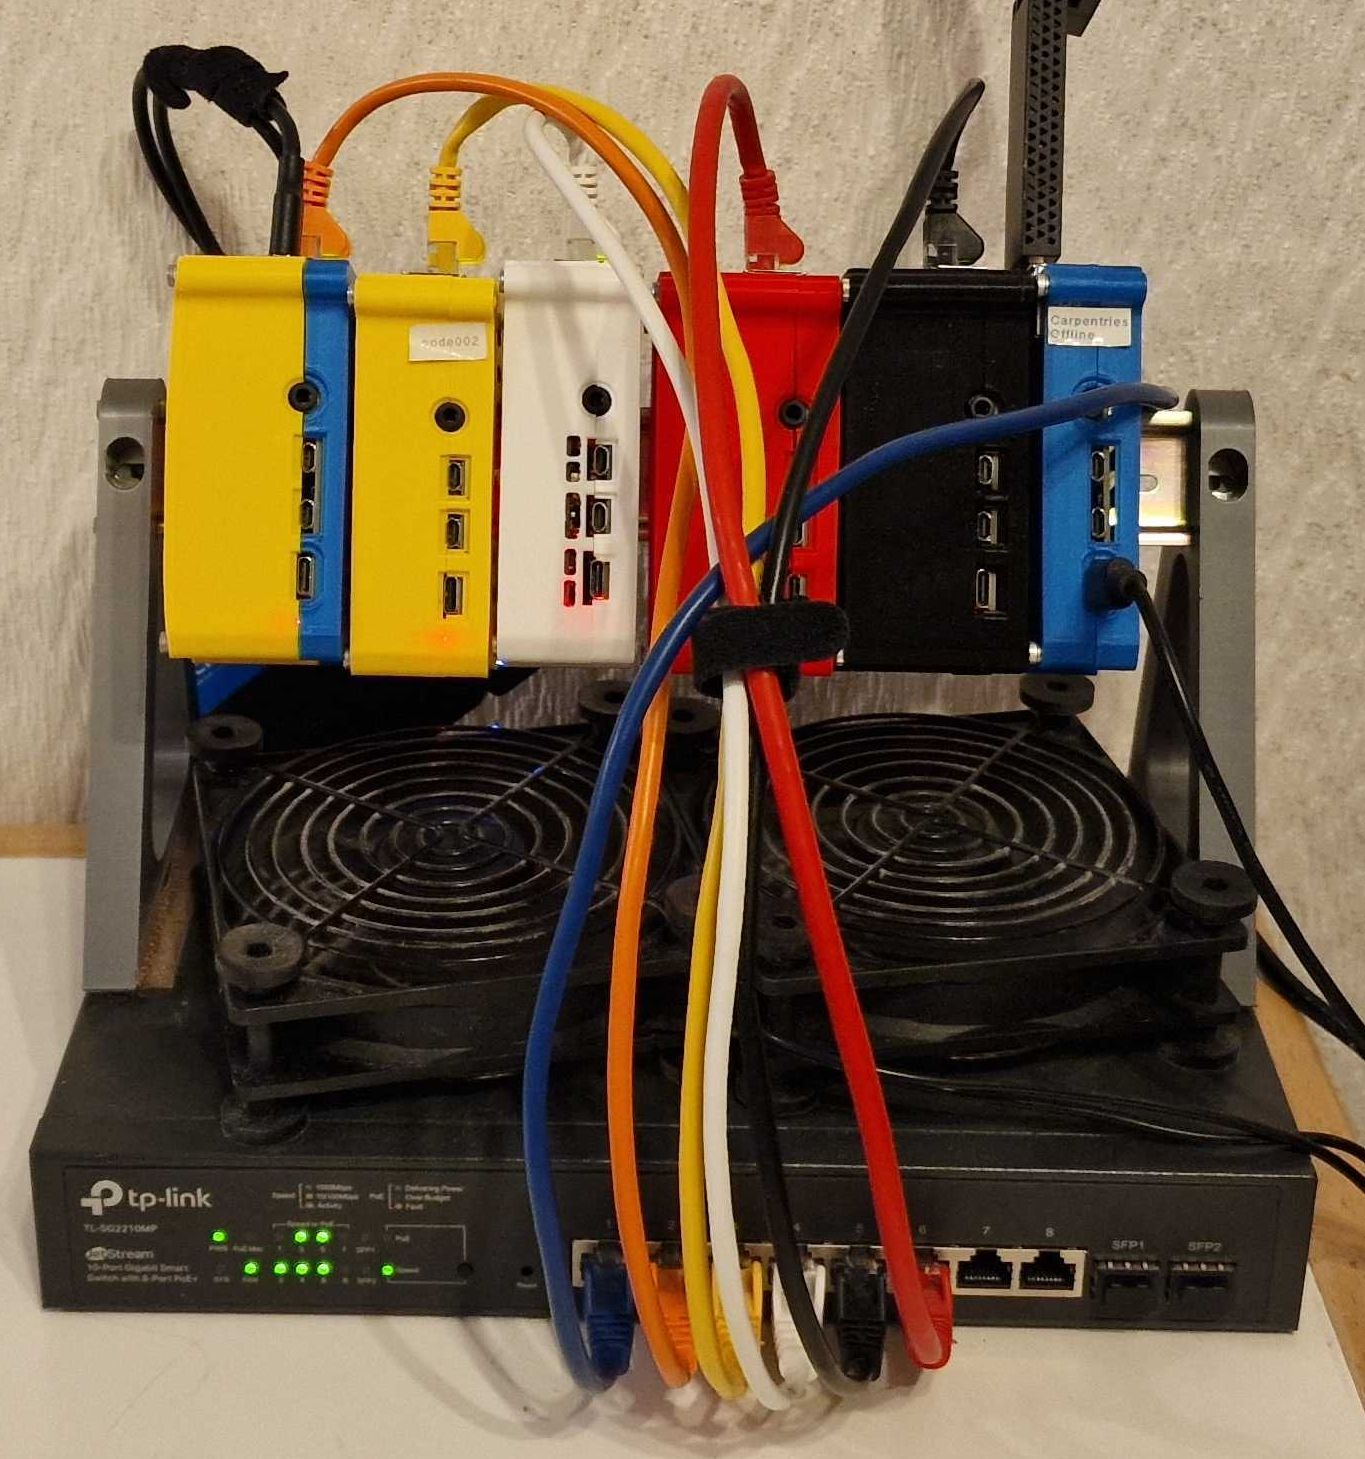
\includegraphics[height=60mm]{pixie.jpg}
	\end{figure}
\end{frame}
\begin{frame}{Why would we need a miniHPC}
	\begin{itemize}

		\item Hardware less abstract.
		\item Real system are busy doing actual research (85 - 95\%) load on systems).
		\item Fear amongst learners that they are going to break the multi-million system they are playing on.
		\item Resource limits more apparent.
		\item More control over the environment.
		\item No need to have accounts on a real HPC.
		\item Own access point, so no need to get people on university network.
	\end{itemize}
\end{frame}
\end{document}
